% Insert after the new structured-comparison subsection.
\subsection{Sensitivity to the Validation Fraction}
\label{sec:revision-validation-fraction}

We test validation fractions of 10\%, 20\%, 30\% and 40\% at
$P\in\{10,30\}$ and SNRs of 0 and 10~dB. The other settings are
$N=32$, $K=3$, RSR $=12$~dB and independently drawn three-to-seven
paths per user. We retain the 100 final updates, 25 updates per candidate
and four Cadzow sweeps. For each pilot-count/SNR pair, the four fractions
use the same 400 channel, pilot and noise realizations. The validation
sets are nested trailing pilot columns. All $P$ pilots are reused for
every final fit, so the comparison changes the rank-selection split
rather than the total transmitted pilot count.

Fig.~\ref{fig:revision-holdout} shows that the split matters. For example,
at $P=30$ and SNR $=10$~dB, using 10\% instead of 30\% gives a paired
ratio-of-sums gain of $-0.602$~dB, with interval
$[-0.832,-0.383]$~dB. At $P=10$ and SNR $=10$~dB, increasing the
fraction from 30\% to 40\% gives $-0.461$~dB
$[-0.744,-0.176]$. Negative values mean that the changed split is worse
than the 30\% reference. Neither a very small nor a larger validation
set is therefore automatically better.

The selected ranks also change. At $P=10$ and SNR $=0$~dB, the median
selected rank falls from three with a 10\% split to one with a 40\%
split. Across all 16 settings, full-rank fallback occurs in 0--1.5\% of
the trials. HS-GS still improves on EM-GS in each setting, but the results
do not identify one validation fraction that is best in all conditions.

\begin{figure*}[!t]
\centering
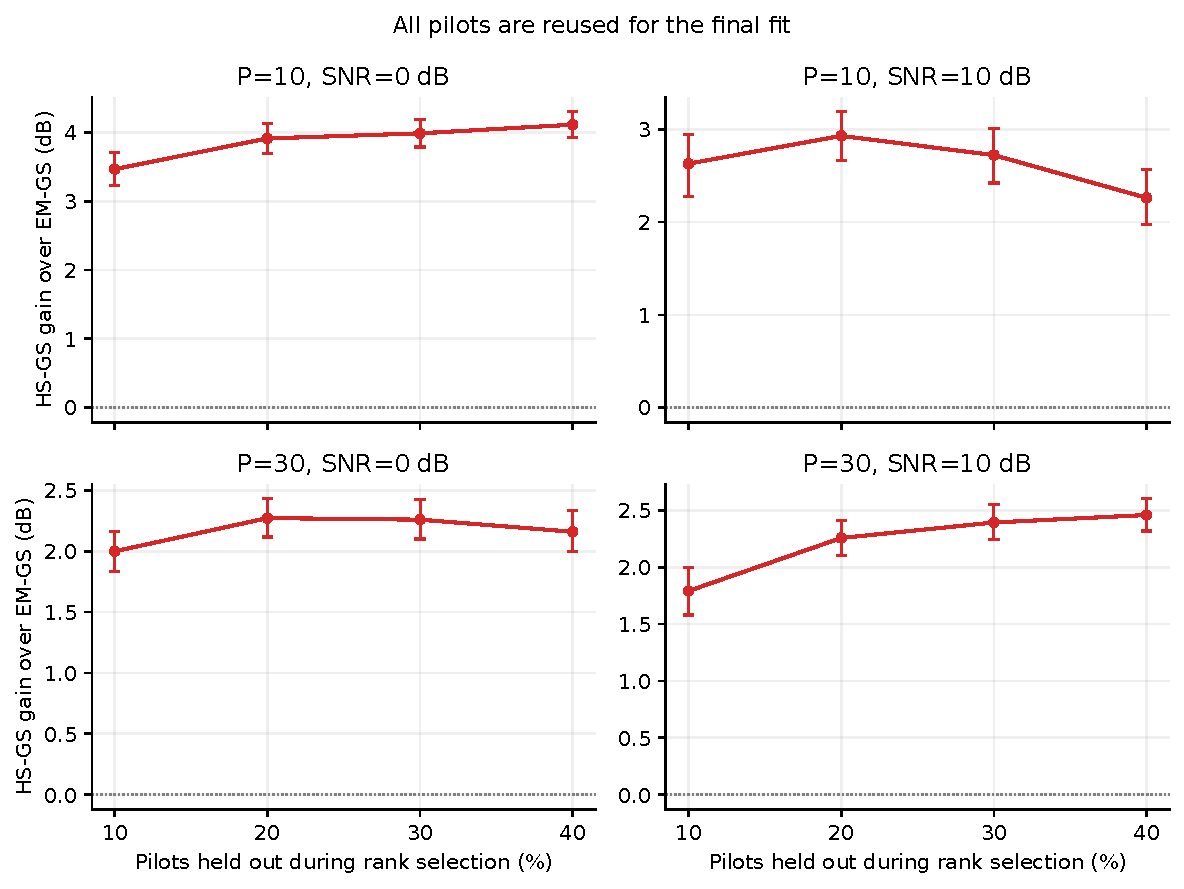
\includegraphics[width=0.90\textwidth]{fig/revision_heldout_fraction.pdf}
\caption{HS-GS ratio-of-sums gain over EM-GS as the validation fraction
changes. The fractions share 400 paired worlds within each panel, and
all pilots are used for the final estimate. Error bars are pointwise
95\% paired-bootstrap intervals from 4,000 resamples.}
\label{fig:revision-holdout}
\end{figure*}
